\documentclass{beamer}

% Top-aligning columns within a top-aligned frame
% https://tex.stackexchange.com/questions/16447/beamer-top-aligning-columns-within-a-top-aligned-frame
\makeatletter
\newenvironment{myitemize}{%
   \setlength{\topsep}{0pt}
   \setlength{\partopsep}{0pt}
   \renewcommand*{\@listi}{\leftmargin\leftmargini \parsep\z@ \topsep\z@ \itemsep\z@}
   \let\@listI\@listi
   \itemize
}{\enditemize}
\makeatother  

\usepackage[USenglish]{babel}
\usepackage[utf8]{inputenc}
\usepackage{amssymb, amsmath}
\usepackage{bm}
\usepackage{color}
\usepackage{tikz}
\usepackage{url}

\definecolor{links}{HTML}{2A1B81}
\hypersetup{colorlinks,linkcolor=,urlcolor=links}

\usetheme{Boadilla}

\bibliographystyle{apalike}
% make bibliography entries smaller
%\renewcommand\bibfont{\scriptsize}
% Now get rid of all the colours
\setbeamercolor*{bibliography entry title}{fg=black}
\setbeamercolor*{bibliography entry author}{fg=black}
\setbeamercolor*{bibliography entry location}{fg=black}
\setbeamercolor*{bibliography entry note}{fg=black}

\newcommand{\lnorm}[1]{\left\lVert#1\right\rVert^2}
\newcommand{\norm}[1]{\left\lVert#1\right\rVert}

% and kill the abominable icon
\setbeamertemplate{bibliography item}{}

\begin{document}
\title[Synthesizer]{Synthesizer: Rethinking Self-Attention in Transformer Models}  
\author{Radek Bartyzal}
\date{26. 5. 2020} 
\institute{GLAMI AI}

\frame{\titlepage} 

%--------- END Frame 12 -------------
\begin{frame}{Motivation}

Transformer uses self-attention:
\begin{itemize}
\item sentence = list of word (token) embeddings of dimension $d$
\item sentence length = number of words = $l$
\item each word is multiplied by Q, K, V $\in \mathbb{R}^{d \times d}$
\item attention vector for word $x$ = $A(x) \in \mathbb{R}^{1 \times l} = Q(x)K(x)^T$
\item attention matrix with row for each word = $A \in \mathbb{R}^{l \times l}$
\item Output = $Y = Softmax(A)G(x)$, G = Value matrix or other function.
\end{itemize}

\vfill
Questions:
\begin{itemize}
\item Is the dot-product of $QK$ = $O(d^3)$ necessary? 
\item replace it by calculating row vectors of $A$ by FF net = don't look at other words?
\item replace it by directly optimizing $A$?
\end{itemize}

\end{frame}

%--------- END Frame 12 -------------
\begin{frame}{Overview}

\begin{figure}[h]
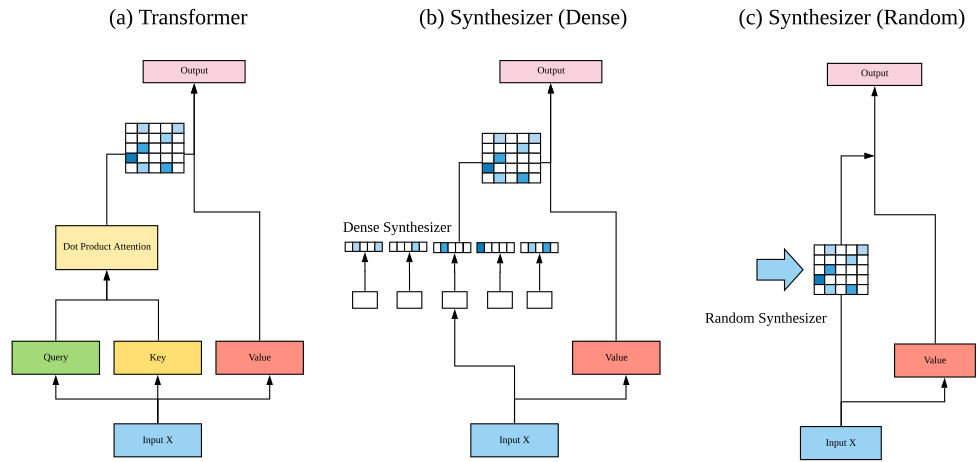
\includegraphics[width=\textwidth]{img/arch}
\caption{Sentence length = 5 words. a) Dot product of $Q, K \in \mathbb{R}^{d \times d}$. \newline b) 2-layer FF applied to each word, no dot product. \newline c) Weight matrix randomly inited $\implies$ optimized or fixed.}
\end{figure}

\end{frame}
%--------- END Frame 12 -------------
\begin{frame}{Overview}
Dense variant adds $d \times l$ params:
\begin{itemize}
\item problem: if $l$ is large that is more than $d^2$
\item solution: factorize the weight matrix to $\mathbb{R}^{d \times a}$ and $\mathbb{R}^{d \times b}$ where $l = ab$
\end{itemize}

\vfill

\begin{figure}[h]
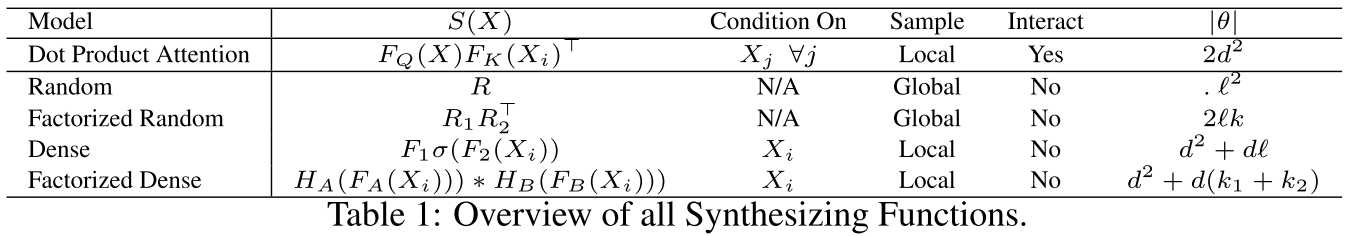
\includegraphics[width=\textwidth]{img/funcs}
\caption{$S(X)$ = Synthesizing function returning $A$ for the whole sentence. Dense variant is conditioned only on each word alone = no interaction with other words.}
\end{figure}

\end{frame}
%--------- END Frame 12 -------------

\begin{frame}{Experiments}

Tasks:
\begin{itemize}
\item machine translation
\item language modeling
\item dialogue generation
\end{itemize}

\vfill

Results:
\begin{itemize}
\item Fixed Random is significantly worse but not complete trash.
\item Both Optimized Random and Dense have competitive results with classic Transformer.
\item Mixing heads from diff. variants helps.
\end{itemize}

\end{frame}

\begin{frame}{Sources}
%--------- END Frame 12 -------------
\begin{thebibliography}{0}

  \bibitem[1]{cit:paper} 1. Tay, Yi, et al. "Synthesizer: Rethinking Self-Attention in Transformer Models." arXiv preprint arXiv:2005.00743 (2020). \url{https://arxiv.org/abs/2005.00743v1} 
  
\end{thebibliography}

\end{frame}

 
\end{document}
